\documentclass[a4paper,11pt]{article}
\input{/home/tof/Documents/Cozy/latex-include/preambule_lua.tex}
\newcommand{\showprof}{show them}  % comment this line if you don't want to see todo environment
\fancyhead[L]{Collection de bandes dessinées}
\newdate{madate}{10}{09}{2020}
%\fancyhead[R]{\displaydate{madate}} %\today
%\fancyhead[R]{Seconde - SNT}
%\fancyhead[R]{Première - NSI}
\fancyhead[R]{Terminale - NSI}
\fancyfoot[L]{~\\Christophe Viroulaud}
\AtEndDocument{\label{lastpage}}
\fancyfoot[C]{\textbf{Page \thepage/\pageref{lastpage}}}
\fancyfoot[R]{\includegraphics[width=2cm,align=t]{/home/tof/Documents/Cozy/latex-include/cc.png}}

\begin{document}
\begin{Form}

\section{Problématique}
Le professeur possède une collection importante de bandes dessinées, qu'il complète régulièrement. Une fois dans sa librairie préférée, il lui arrive de ne plus se souvenir où il en est exactement dans ses séries. De plus il prête régulièrement des livres à ses amis et aimerait pouvoir maintenir à jour l'état de ses étagères.
\begin{figure}[!h]
\centering

\includegraphics[width=3cm]{ressources/biblio.jpg}
\captionof{figure}{Bibliothèque}
\label{biblio}
\end{figure}

\begin{center}
\shadowbox{\parbox{17cm}{\centering Quelle solution peut-on mettre en place pour gérer efficacement la collection de bandes dessinées?}}
\end{center}
\section{Première approche}
La première approche imaginée consiste en l'utilisation d'un tableur (figure \ref{tableur}) pour stocker les informations.
\begin{figure}[!h]
\centering
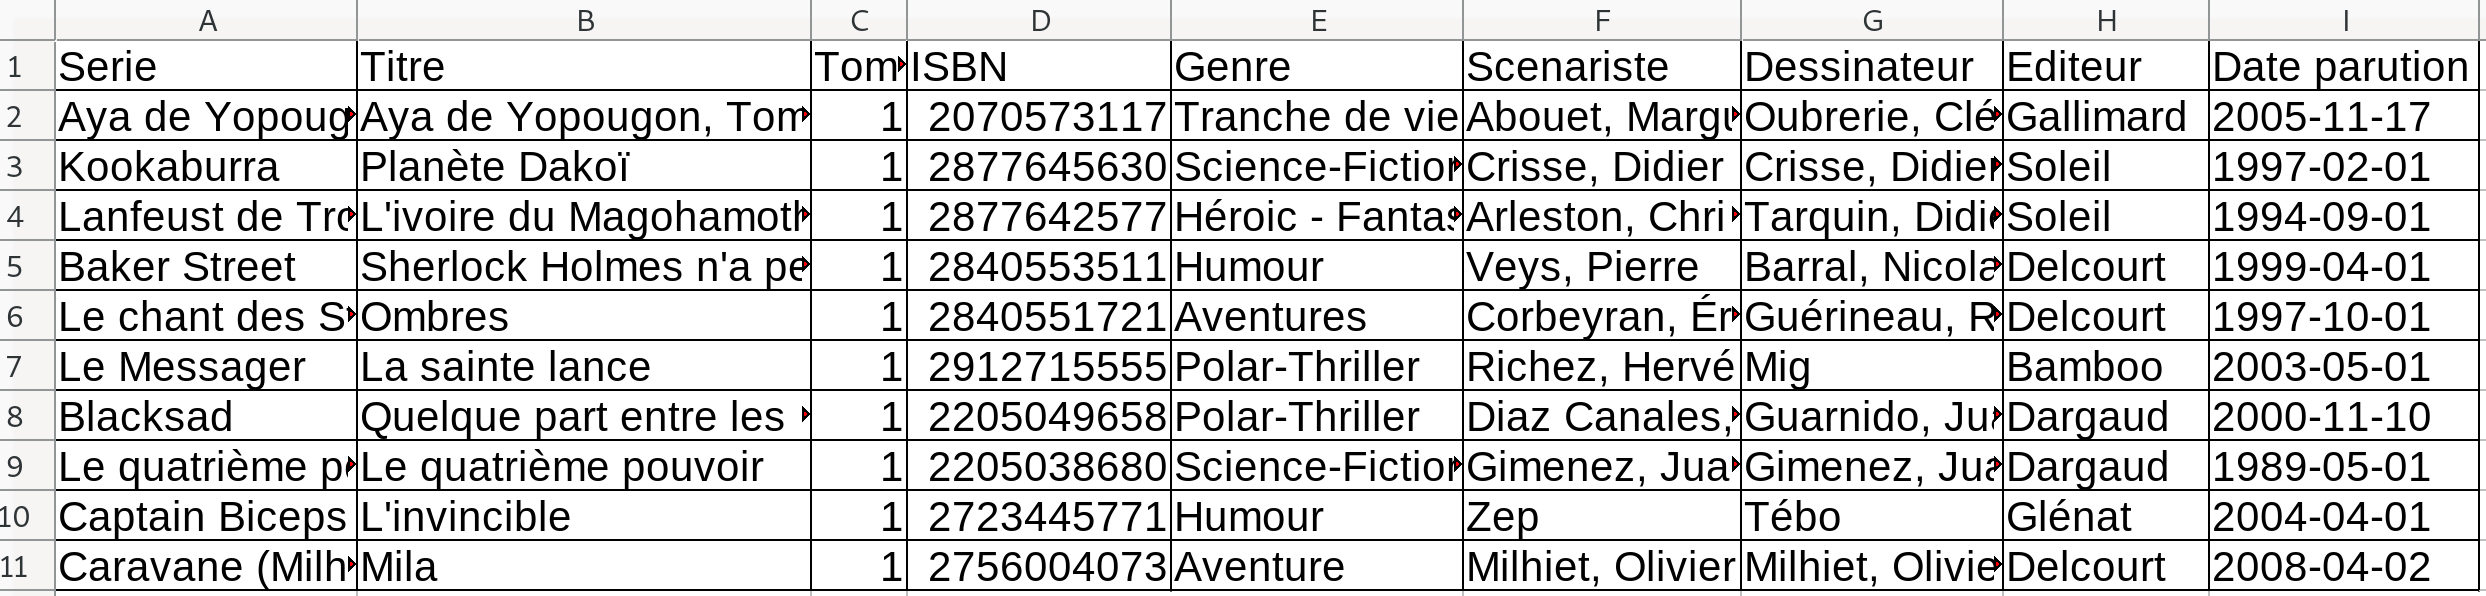
\includegraphics[width=15cm]{ressources/approche-1.png}
\captionof{figure}{Utilisation d'un tableur}
\label{tableur}
\end{figure}

Dans ce tableau, l'ajout d'une colonne \emph{emprunteur} permettrait de gérer les prêts.
\begin{activite}
Établir les limites de cette approche.
\end{activite}
\begin{commentprof}
\begin{itemize}
\item 2000 entrées = gérables par Python, mais si on veut étendre notre système à structure plus importante?
\item comment gérer modifications efficacement (ex: changement titre d'une série?)
\item pb tableur $\;\rightarrow\;$ article "malades du covid oubliés"
\item Si on veut plus d'infos sur l'emprunteur (nom, date anniversaire), les colonnes ajoutées sont-elles pertinentes dans ce tableau? Quand il rend un livre il faut vérifier/modifier beaucoup de lignes.
\item Que se passe-t-il si on change le titre d'une BD? L'emprunteur a-t-il vraiment pris ce livre?
\end{itemize}
\end{commentprof}
\section{Modèle de données}
\subsection{Modèle relationnel}
La première étape est de définir la manière dont les données vont être représentées. Le \emph{modèle relationnel} est un des plus populaires. Dans ce modèle théorique:
\begin{itemize}
\item Une \textbf{entité} est un objet représenté par un n-uplet de valeurs scalaires. Une bande dessinée est une \emph{entité}:
\begin{center}
(Captain Biceps, L'invincible, 1, 2723445771, Humour, Zep, Tébo, Glénat, 2004-04-01)
\end{center}
\item Une \textbf{relation} est l'ensemble des entités. On parle aussi de \emph{table}. La collection  de bandes dessinées est une \emph{relation}:
\begin{center}
(Captain Biceps, L'invincible, 1, 2723445771, Humour, Zep, Tébo, Glénat, 2004-04-01),\\
\small{(Caravane, Mila, 1, 2756004073, Aventure, Milhiet Olivier, Milhiet Olivier, Delcourt, 2008-04-02)},\\
(Kick-Ass, Le premier vrai super-héros, 1, 2809409994, Comics, Millar Mark, Romita Jr John, Panini Comics, 2010-03-17)

\end{center}
\item Une \emph{relation} possède des \textbf{attributs}. La relation des bandes dessinées possède les attributs:
\begin{center}
(serie, titre, tome, isbn, genre, scenariste, dessinateur, editeur, date\_parution)
\end{center}
\item Chacun de ces attributs est défini dans un domaine.
\begin{center}
\begin{tabular}{|cc|}
\hline 
\multicolumn{2}{|c|}{Bandes\_dessinees} \\ 
\hline 
serie & String \\ 
titre & String \\ 
tome & Integer \\ 
isbn & Integer \\ 
genre & String \\ 
scenariste & String \\ 
dessinateur & String \\ 
editeur & String \\ 
date\_parution & Date \\ 
\hline 
\end{tabular} 
\captionof{code}{\textbf{Schéma} de la relation bandes\_dessinees}
\end{center}
Une autre manière de présenter le schéma:

Bandes\_dessinees(serie \emph{String}, titre \emph{String}, tome \emph{Integer}, isbn \emph{String}, genre \emph{String}, scenariste \emph{String}, dessinateur \emph{String}, editeur \emph{String}, date\_parution \emph{Date})
\end{itemize}
\begin{commentprof}
scalaire = atomique; définit par un type "de base"$\;\rightarrow\;$carte d'identité d'une personne n'est pas une donnée scalaire. 
\end{commentprof}
\begin{activite}
\begin{enumerate}
\item Sur le même modèle définir la relation des Emprunteurs.
\item Les relations actuelles permettent-elles de gérer les emprunts? Quelle solution mettre en place?
\end{enumerate}
\end{activite}
\begin{commentprof}
table Emprunteurs: impossible de mettre les emprunts dedans $\;\rightarrow\;$le mettre en évidence
questionnement:
\begin{itemize}
\item si noms emprunteurs communs (dans Emprunteurs)? $\rightarrow$ contrainte d'entité
\item comment s'assurer qu'on n'a pas mis 2 fois le même emprunt dans la table (par erreur)? $\rightarrow$ contrainte d'entité (isbn = clé primaire Emprunts)
\item si on retire un emprunteur (n'est plus mon ami)? il risque d'y avoir des bd non rendues $\rightarrow$ contrainte de référence
\end{itemize}
\end{commentprof}
\subsection{Contraintes d'intégrité}
Une contrainte d'intégrité est une propriété vérifiée à tout instant et qui garantit \emph{la cohérence des données}.
\subsubsection{Contrainte de domaine}
Chaque propriété que l'on souhaite renseigner est représentée par un \emph{attribut} dans une relation. Le \emph{domaine de définition} de chaque attribut doit garantir qu'il n'y aura pas de perte de données.
\begin{activite}
Ajouter l'attribut \emph{telephone} dans la relation \emph{Emprunteurs}. Quel domaine de définition semble le plus approprié?
\end{activite}
\begin{commentprof}
telephone $\;\rightarrow\;$Integer? risque de perdre info (le 0 du début) et certains affichages commencent par +33 $\;\rightarrow\;$String plus approprié

équivalent type de données en Python

autre exemple: une variable binaire (oui/non) $\;\rightarrow\;$ la représenter par un booléen garantit qu'il ne pourra pas y avoir de 3° choix.
\end{commentprof}
\subsubsection{Contrainte d'entité}
Elle garantit que chaque entité d'une relation est \emph{unique} et l'identifie de manière non ambiguë. Lors de la modélisation, il faut s'assurer qu'un attribut (ou un ensemble d'attributs) permet d'identifier l'entité de manière unique.
\begin{activite}
Dans la relation \emph{Bandes\_dessinees}, y-a-t-il un attribut qui garantit cette contrainte?
\begin{commentprof}
dans une première approche isbn, même si: isbn-10 et isbn-13 et certains isbn ont des lettres. \sout{De plus le csv fournit ne contient pas tous les isbn}
\end{commentprof}
\end{activite}
\begin{aretenir}[]
On appelle \textbf{clé primaire} l'attribut qui garantit l'unicité de l'entité.
\end{aretenir}
On indique la \emph{clé primaire} en la soulignant dans le schéma:\\
Bandes\_dessinees(serie \emph{String}, titre \emph{String}, tome \emph{Integer}, \underline{isbn \emph{String}}, genre \emph{String}, scenariste \emph{String}, dessinateur \emph{String}, editeur \emph{String}, date\_parution \emph{Date})
\begin{activite}
\begin{enumerate}
\item Dans la relation \emph{Emprunteurs} l'attribut \emph{nom} permet-il de garantir cette contrainte?
\item Quelle solution peut-on mettre en place?
\end{enumerate}
\begin{commentprof}
ensemble nom-prenom pas suffisant non plus: il existe plusieurs  Christophe Viroulaud
\end{commentprof}
\end{activite}
\subsubsection{Contrainte de référence}
Elle crée des associations entre deux relations. Elle garantit qu'une entité d'une relation B mentionne une entité existante dans une relation A.
\begin{activite}
\begin{enumerate}
\item Dans l'encadré ci-après, écrire à nouveau la relation \emph{Emprunts} en utilisant les clés primaires des autres relations.
\item Définir une clé primaire pour cette relation.
\end{enumerate}
\end{activite}
\begin{framed}
Emprunts(
\end{framed}

\begin{commentprof}
compléter le schéma dans l'encadré; les clés étrangères en pointillés\\
Emprunts(\underline{\dashuline{isbn Integer}}, \dashuline{id\_emprunteurs Integer})\\
Les attributs \emph{isbn} et \emph{id\_emprunteurs} sont des \textbf{clés étrangères}. Cela signifie que la valeur de l'attribut \emph{isbn} dans la relation \emph{Emprunts} doit être une valeur existante dans la relation \emph{Bandes\_dessinees}. De même la valeur de l'attribut \emph{id\_emprunteurs} dans la relation \emph{Emprunts} doit être une valeur existante  de \emph{id} dans la relation \emph{Emprunteurs}.\\
il n'est pas obligatoire que la clé étrangère ait le même nom que la clé primaire correspondante\\
isbn est également clé primaire de la relation: on ne peut prêter 2 fois le même livre; id\_emprunteurs pas possible car une même personne peut prendre plusieurs bd
\end{commentprof}
\begin{aretenir}[]
Une \textbf{clé étrangère} est une référence à une clé primaire d'une autre relation. Elle garantit:
\begin{itemize}
\item que la valeur de l'attribut crée dans la relation existe dans la relation liée,
\item qu'on ne peut supprimer une entité si elle est liée à une autre relation.
\begin{commentprof}
on ne peut supprimer un emprunteur s'il a encore des emprunts
\end{commentprof}
\end{itemize}
\end{aretenir}
\begin{commentprof}
\subsubsection{Contrainte utilisateurs}
ou contraintes métiers: spécifiques à la modélisation (exemple email ne contient que 1@, âge < 200)
\end{commentprof}
\section{Base de données}
\begin{aretenir}[]
L'ensemble des relations constitue une \textbf{base de données}.
\end{aretenir}
\begin{figure}[!h]
\centering
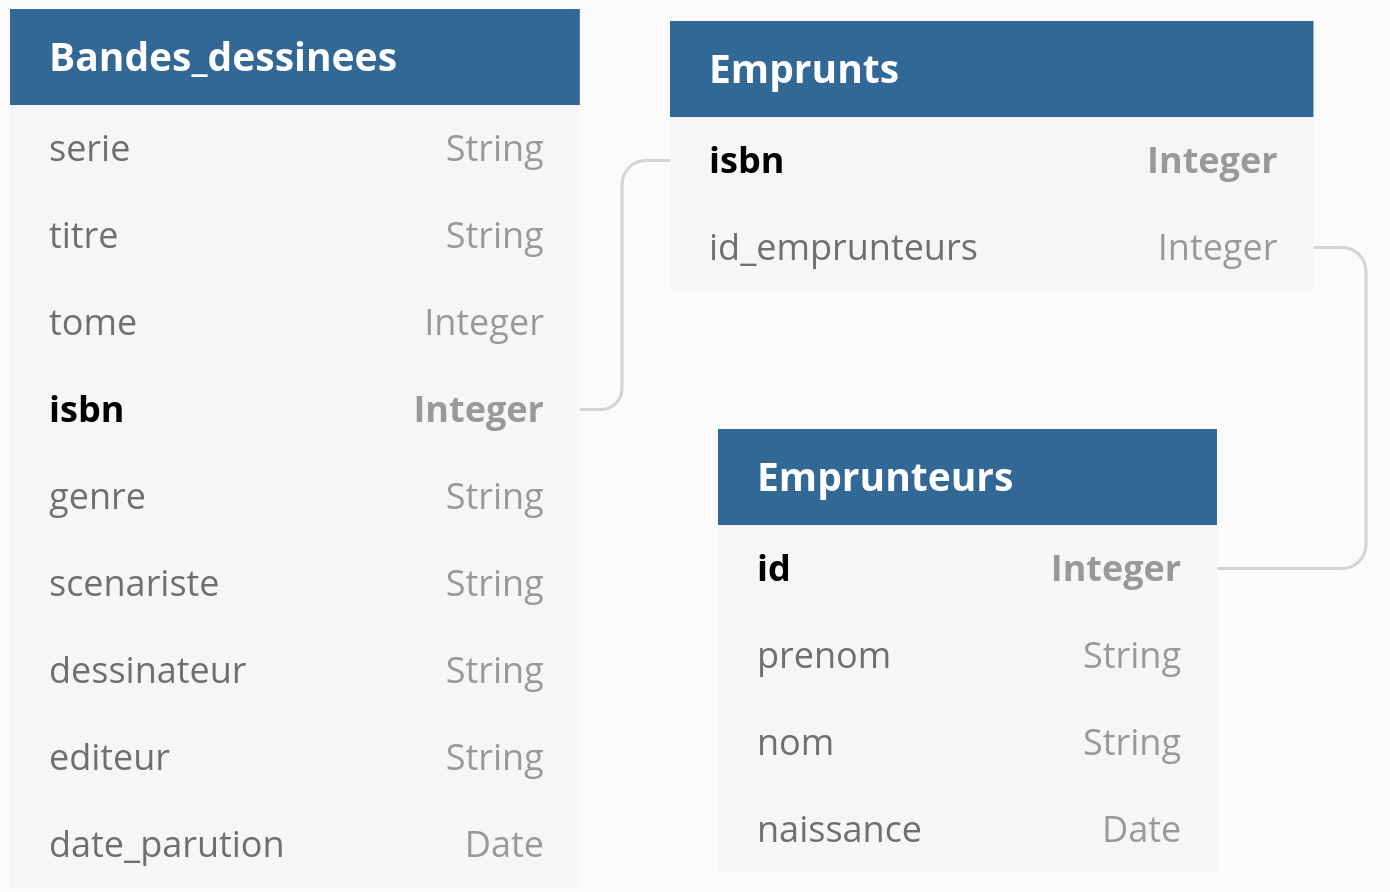
\includegraphics[width=12cm]{ressources/cle_etrangere.png}
\captionof{figure}{Base de données}
\label{bdd}
\end{figure}
\begin{commentprof}
Les 2 attributs de Emprunts sont des clés étrangères
\end{commentprof}
\begin{activite}
Cette construction peut être améliorée. En effet, un même éditeur publie de nombreuses bandes dessinées.
\begin{enumerate}
\item Modifier la base de données pour prendre en compte cette observation.
\item D'autres attributs de la relation \emph{Bandes\_dessinees} répondent au même constat. Proposer une nouvelle version de la base de données.
\end{enumerate}
\begin{commentprof}
id\_dessinateur et id\_scenariste sont \textbf{des clés étrangères} de l'attribut id de Auteurs (et pas l'inverse): on peut créer un auteur qui n'a pas encore écrit de bd mais on ne peut pas créer une bd qui n'a pas d'auteur référencé.\\
Idem pour id\_genre et id\_editeur
\end{commentprof}
\end{activite}
\end{Form}
\end{document}